
\section{From Data Breach to Identity Theft}
\label{sec:breach_to_victim}

%\com{I took out the thetas in the equations because in the bullet point for $r_t$, we say scaled by theta so it's already included. Or if you think it's more clear, we can move the theta out of the bullet point and into the numerator of the equation.}

% To see how the model compounds, we can expand the formula for the first few years. \rev{At $t=0$, the start of 2008, we have the initial condition $C_0 = 0$, which implies $\mu_0 = 0$. For the first year $t=1$, the number of newly unique records is $c_1 = r_1 \times \gamma_0(1-\mu_0) = r_1 \gamma_0$. The number of cumulative unique records at the end of the first year is then $C_1 = c_1$. For the second year $t=2$, we calculate the saturation $\mu_1 = \frac{C_1}{N_1 \theta}$, leading to a density of $\gamma_2 = \gamma_0 (1-\mu_1)$. Then, the number of new unique cumulative records for the second year is $c_2 = r_2 \times \gamma_0(1-\mu_1)$, and so on.} \com{See my comment in email that we need not treat 2008 as $t=0$, but maybe it is irrelevant.. this being a geometric sequence it really doesn't matter where we start as?} \resp{Yes that makes sense. I don't think it matters, it would just shift the model to saturation faster.}

%\com{What do you use as the initial value $r_0$?} \resp{I used the number of raw records in 2008, but under our new indexing, that should be $r_1$, see updated above.}

% In our model, we cap the saturation index $\mu_t$ at 95\%, following the assumption that in a modern digital economy, 100\% saturation is never truly achieved due to new entrants (e.g. individuals turning 16), and the constant creation of new identifiers such as email addresses and credit cards. The 5\% buffer in our model ensures that we always account for a small amount of new data entering the digital market. If we reached full saturation, the term $(1-\mu_t)$ would become 0, and if $\mu_t >1$, the term would become negative. This would result in 0 or negative identity discovery, which is not likely in a growing economy.
%\com{So I agree that $\mu$ should not exceed 1 (or else we need to tweak the model. I have two questions here: (1) what about your argument that the same individual could have multiple records? Wouldn't that mean $C_t$ ultimately could be a multiple of $N_t$ and $\mu$ then exceed 1? We may need to revise what we mean by ``unique record''. (2) what do you mean by capping the saturation at 95\%? Doesn't the model automatically update this quantity over and over and we can't just force it to be a certain number, can we?  On the same note, I was going to suggest that if you assume $R$ is the same every year, and $N$ never changes, then you should be able to see whether $\mu$ and these other quantities converge and if so what the limiting values are, correct?}

% \resp{By unique records I meant that one person could have more than one unique record. For example I could have 4 unique records, being my email, SSN, credit card number, and bank account number. Therefore a unique record does not mean a unique identity. That is true that $C_t$ is a multiple of $N_t$ and the $\mu$ exceeds one. In this model the $\mu$ begins to exceed 1 at 2016... that's why I capped it or else the model would break. If you don't think that's valid, then maybe this model is flawed and we should consider a new one? It's true that the the $\mu$ keeps updating iteratively, but i didn't see it converge until I capped it... it just kept growing because the number of leaked records kept growing and growing, much faster than the population. I have some more ideas for a better model. We can discuss today. }

% Analysis of our model showed that the U.S. market reached the 95\% saturation threshold by 2016. By 2021, the cumulative number of estimated unique records $C_t$ reached around 693 million, roughly 2.65 times larger than the U.S. population in 2021. This could be attributed to the fact that a single person often has multiple different records that could identify them, such as multiple email addresses, credit cards, and other accounts. 

% According to a 2017 report by the IDT Resource Center and CyberScout \cite{ITRC_2016_Breach}, the data landscape of 2016 represented a "point of no return for millions of Americans." The report also mentions that in 2016, over half of the data breaches tracked by ITRC contained Social Security Numbers (SSNs) \cite{ITRC_2016_Breach}. Because SSNs are permanent identifiers that cannot be cycled like credit card numbers, this suggests that by 2016, the number of exposed records was approaching saturation. This theory is also confirmed by the collapse in the black market value of identity data. According to \citet{Opderbeck2023}, the market for a complete identity profile decreased from a high of \$150 in 2007 to \$1.50 in 2016, due to what they mention as "an astonishing 99\% decrease apparently resulting from market saturation" \cite{Opderbeck2023, Steel2019}.




% We define a year-specific coefficient, $\gamma_t = \gamma_0 \times (1 - \mu_t)$. Here, $\gamma_0 = 0.8$ represents the base identity density\com{defined how...?}, and $\mu_t$ represents the saturation index, which we define as the ratio of cumulative unique records exposed to the total U.S. population aged 16 and older \cite{FRED_Population}. We utilized annual population estimates from the U.S. Bureau of Labor Statistics \cite{FRED_Population} to calibrate $\mu_t$, accounting for the growth in population between 2008 and 2021. This dynamic adjustment ensures that the model accounts for de-duplication, because a record exposed in 2021 is more likely to be redundant than one exposed in 2008.} For massive breaches, such as the Target or Equifax breaches, we applied an additional overlap discount of $0.8$ to model the high probability that these massive data breaches contain redundant information for individuals already present in the national supply. This provided us with an estimate of the number of records exposed over time. 

% This estimate of the number of unique records exposed over time served as an interesting comparison with the timeline of successful IDTs from the ITS data. This led us to the calculation of the breach to IDT victim conversion rate, defined as the number of IDT victims per 100,000 exposed records. By applying a six-month rolling average to this rate, we smoothed the volatility of individual breach events to identify long-term trends in how effectively criminals convert compromised data into successful IDT, providing insight to the volume of record exposure and resulting social harm. 
% \com{This is very good. Two additional thoughts on this: (1) is there any way we can try to calibrate/verify this method (the formula complete with our choice of the constant values on someone else's dataset, and see if there is a reasonable match? (2) what if we compound $\gamma$ with each passing year while adjusting for the growth of the adult population in the US, to reflect that over time there is perhaps more and more overlap... if you thinks this conjecture makes sense?}
% \resp{(1) Yes, we could start by comparing the $n_u$ (number of estimated undisclosed records breached) to what the Graves credit card paper found. This is what we used regression for from Section \ref{sec:PRC_processing}. We estimated an additional 2,445,160 records annually. They estimated 630,000 records annually. Our is about 4x as much, which I think is reasonable because they only consider credit cards while we consider all forms of records, and they only consider years up to 2014 while we consider up to 2021. Also see the new additions to Section \ref{sec:PRC_processing}.
% (2) I think this makes sense, we could do something like $\gamma_t = \gamma_0 \times (1-\mu_t)$, where $\mu_t$ represents the saturation relative to total US population. This would reflect that a breach in 2021 is more likely to contain redundant information than a breach in 2008. See edits above and see updated plots in Section \ref{sec:data_breach}.}

%\com{So, if I am looking at Fig 7 correctly, the green (actual cases of theft) seems to track the orange (estimated cases of exposure) fairly well, correct? If so this would be very interesting and would be strong evidence of the validity of the model.. as well as a strong argument that corporate data breaches do lead to ID thefts.  One more suggestion is to add annotations to Fig 7 indicating the timing of a set of mega breaches... One can also test the hypothesis whether there is a statistically significant uptick in IDT following a major breach event...}



In what follows, we will (1) perform a statistical test to see in what sense a major breach event may be directly correlated with a subsequence increase in reported IDT incidents, and (2) present a model that estimates a ``breach-to-victim'' conversion rate. These are then used to perform a lower-bound and an upper-bound estimate on the social cost of given major breach events, respectively.

\subsection{Testing Whether There is an Increase in IDT Following a Mega-Breach}
\label{sec:wilcoxon_methods}

To analyze the relationship between large scale data breaches and subsequent IDT victimization, we conduct a Wilcoxon signed-rank test \cite{conover1999practical}. Here we define a ``mega-breach'' as a breach that exposes at least 10 million records. For this experiment, we utilize both the augmented PRC data as well as the processed ITS data. %The PRC data breach chronology (augmented with HHS filings and incidents reported by state-level sources, as discussed in Section \ref{sec:PRC_processing})
The former is used exclusively to identify the time stamps of mega-breaches, while the later serves as the metric to measure the actual change in victimization levels. Essentially, the PRC data marks the events in time, allowing us to align the ITS victim reports into ``pre-breach'' and ``post-breach'' windows for statistical comparison. 

A Wilcoxon signed-rank test was selected to test whether or not the months following a mega-breach exhibit a statistically significant increase in the number of reported IDTs. This test was chosen due to outliers in the data that violate the normality assumptions required for t-tests. To satisfy the Wilcoxon requirement for independent pairs of observations, breaches occurring within 3 months of one another were treated as a single compound event. In such instances, the event month $T_0$ is defined as the month of the initial breach in the cluster. This consolidation resulted in 19 distinct mega-breach events identified in the augmented PRC data.

We used a fixed six month window ($T_0-6$ to $T_0-1$) to measure the baseline median victimization level prior to each mega-breach. Because IDT is rarely discovered at the exact moment of a breach, we conducted a longitudinal sweep across varying ``discovery lags'' ($i$), which we define as the time delay (in months) between data exposure (marked by PRC) and IDT discovery (measured by ITS). Each choice of the $i$ value then defines a ``post-breach'' window of 6 months. For example, if a mega-breach event occurred in May, and if we consider a 1-month discovery lag, then any IDT occurring between June and November of that year would fall into the post-breach window. 

We consider a range of possible discovery lags, $i \in \{0, \dots, 8\}$, and for each value $i$ we compared the pre-breach baseline to the six-month post-breach observation window starting at $T_0 + i$. For each discovery lag value, we performed the Wilcoxon signed-rank test for the following hypotheses:

% Our experiment tested discovery lag values between 1 to 8 months. For each discovery lag value $i$, we considered an observation window of six months, delayed by $i$ months to measure our post-breach number of victims.  

% To account for the potential lag between corporate exposure and IDT discovery, we consider a six month observation window. We test the following:, following the definition of a mega-breach in the 2024 IBM Cost of a Data Breach Report \cite{ibm_cost_breach_2024}

\begin{enumerate}
    \item $H_0$ (Null Hypothesis): The median rate of IDT discovery in the six-month window following a mega-breach (delayed by lag $i$) is not significantly higher than the median rate in the six-months preceding it.
    \item $H_1$ (Alternate Hypothesis): The median rate of IDT discovery in the six-month window following a mega-breach (delayed by lag $i$) is significantly higher than the median rate in the six-months preceding it.
\end{enumerate}



% We executed this experiment twice to evaluate our dynamic saturation model. Thus, this experiment was run on both the raw but augmented PRC breach chronology data (augmented with HHS and state-level data), as well as on the output of our dynamic saturation model, which attempted to de-duplicate the raw PRC data breach chronology data.  
% The results of testing discovery windows of $i \in \{1, \dots, 8\}$ are shown in Figure \ref{fig:wilcoxon_raw}, which shows the results for the testing done on the raw PRC data breach chronology data, and Figure \ref{fig:wilcoxon_saturated}, which shows the results for the testing done on the data after our dynamic saturation model was applied. In both of these plots, the blue line tracks the $p$-value across varying discovery lags, while the green bars indicate the average change in the estimated number of victims monthly, from 6 months before the breach and $i$ months after.

\begin{figure}[htbp]
    \centering
    % First Subfigure (Original Data)
    \begin{subfigure}[b]{0.48\textwidth}
        \centering
        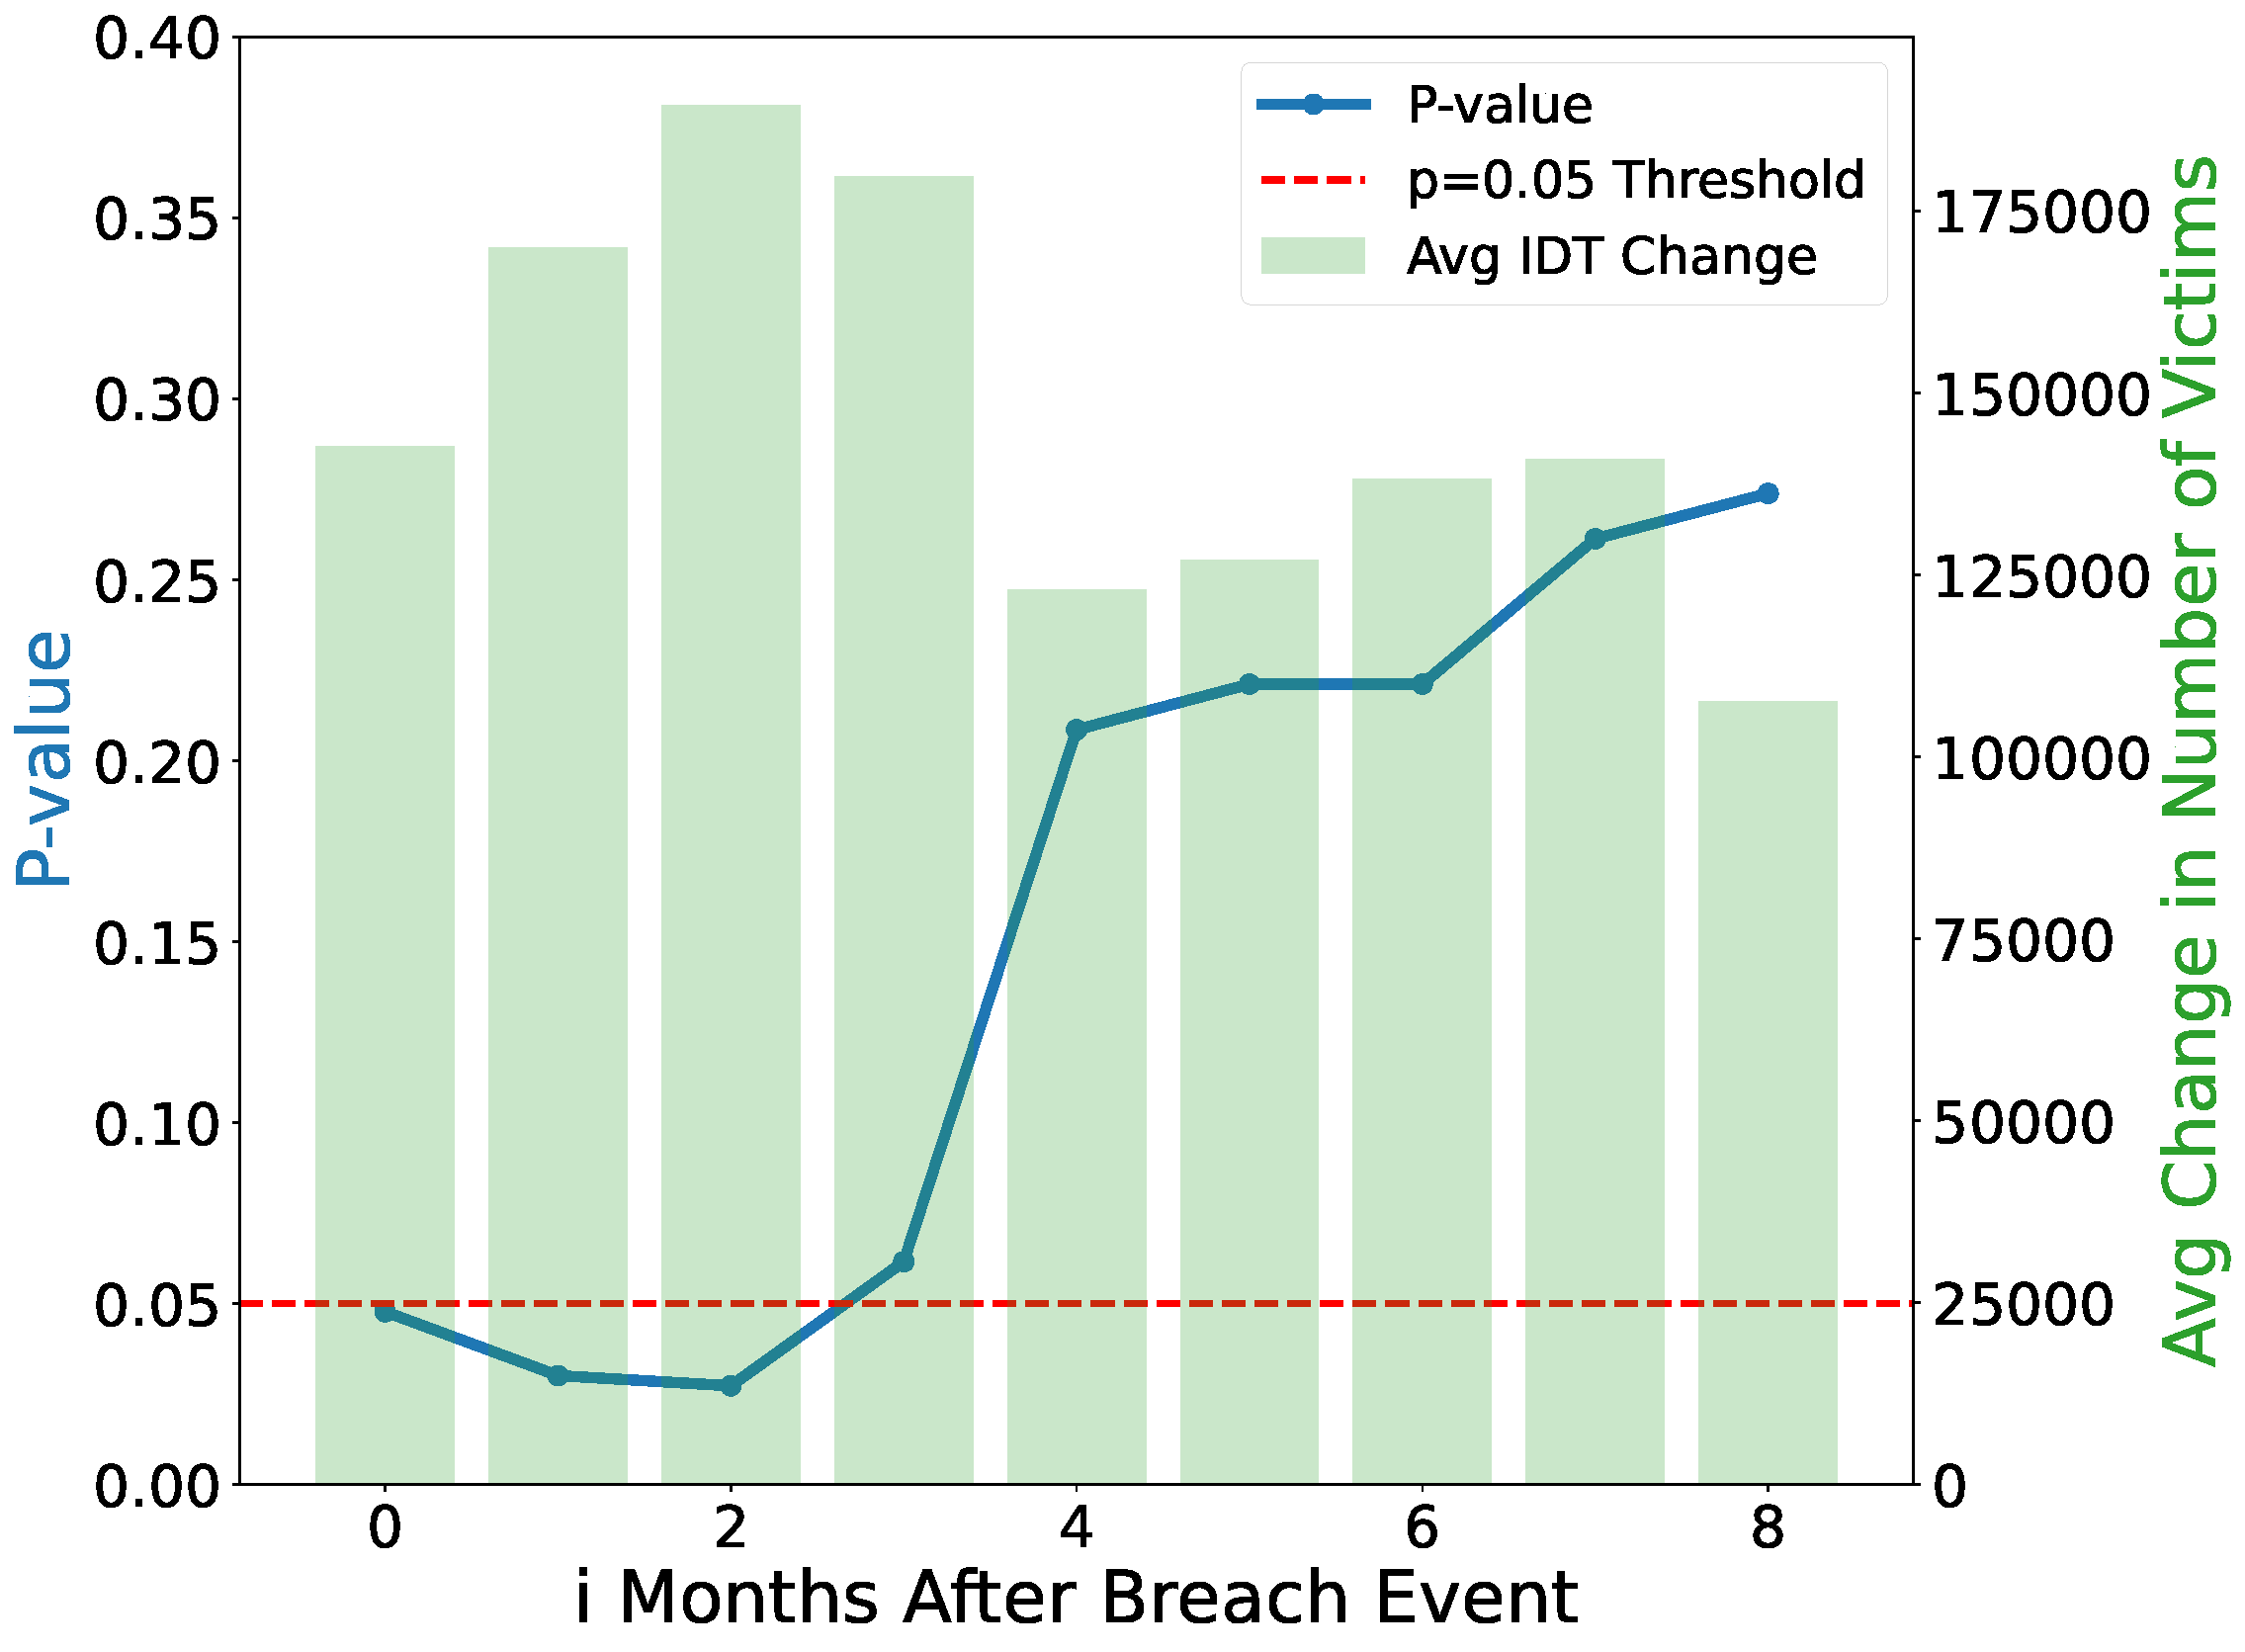
\includegraphics[width=\textwidth]{figures/part6/longitudinal_sweep_raw_data.pdf}
        \caption{Augmented PRC data.}
        \label{fig:wilcoxon_raw}
    \end{subfigure}
    \hfill % Adds horizontal space between the two images
    % Second Subfigure (Placebo Data)
    \begin{subfigure}[b]{0.48\textwidth}
        \centering
        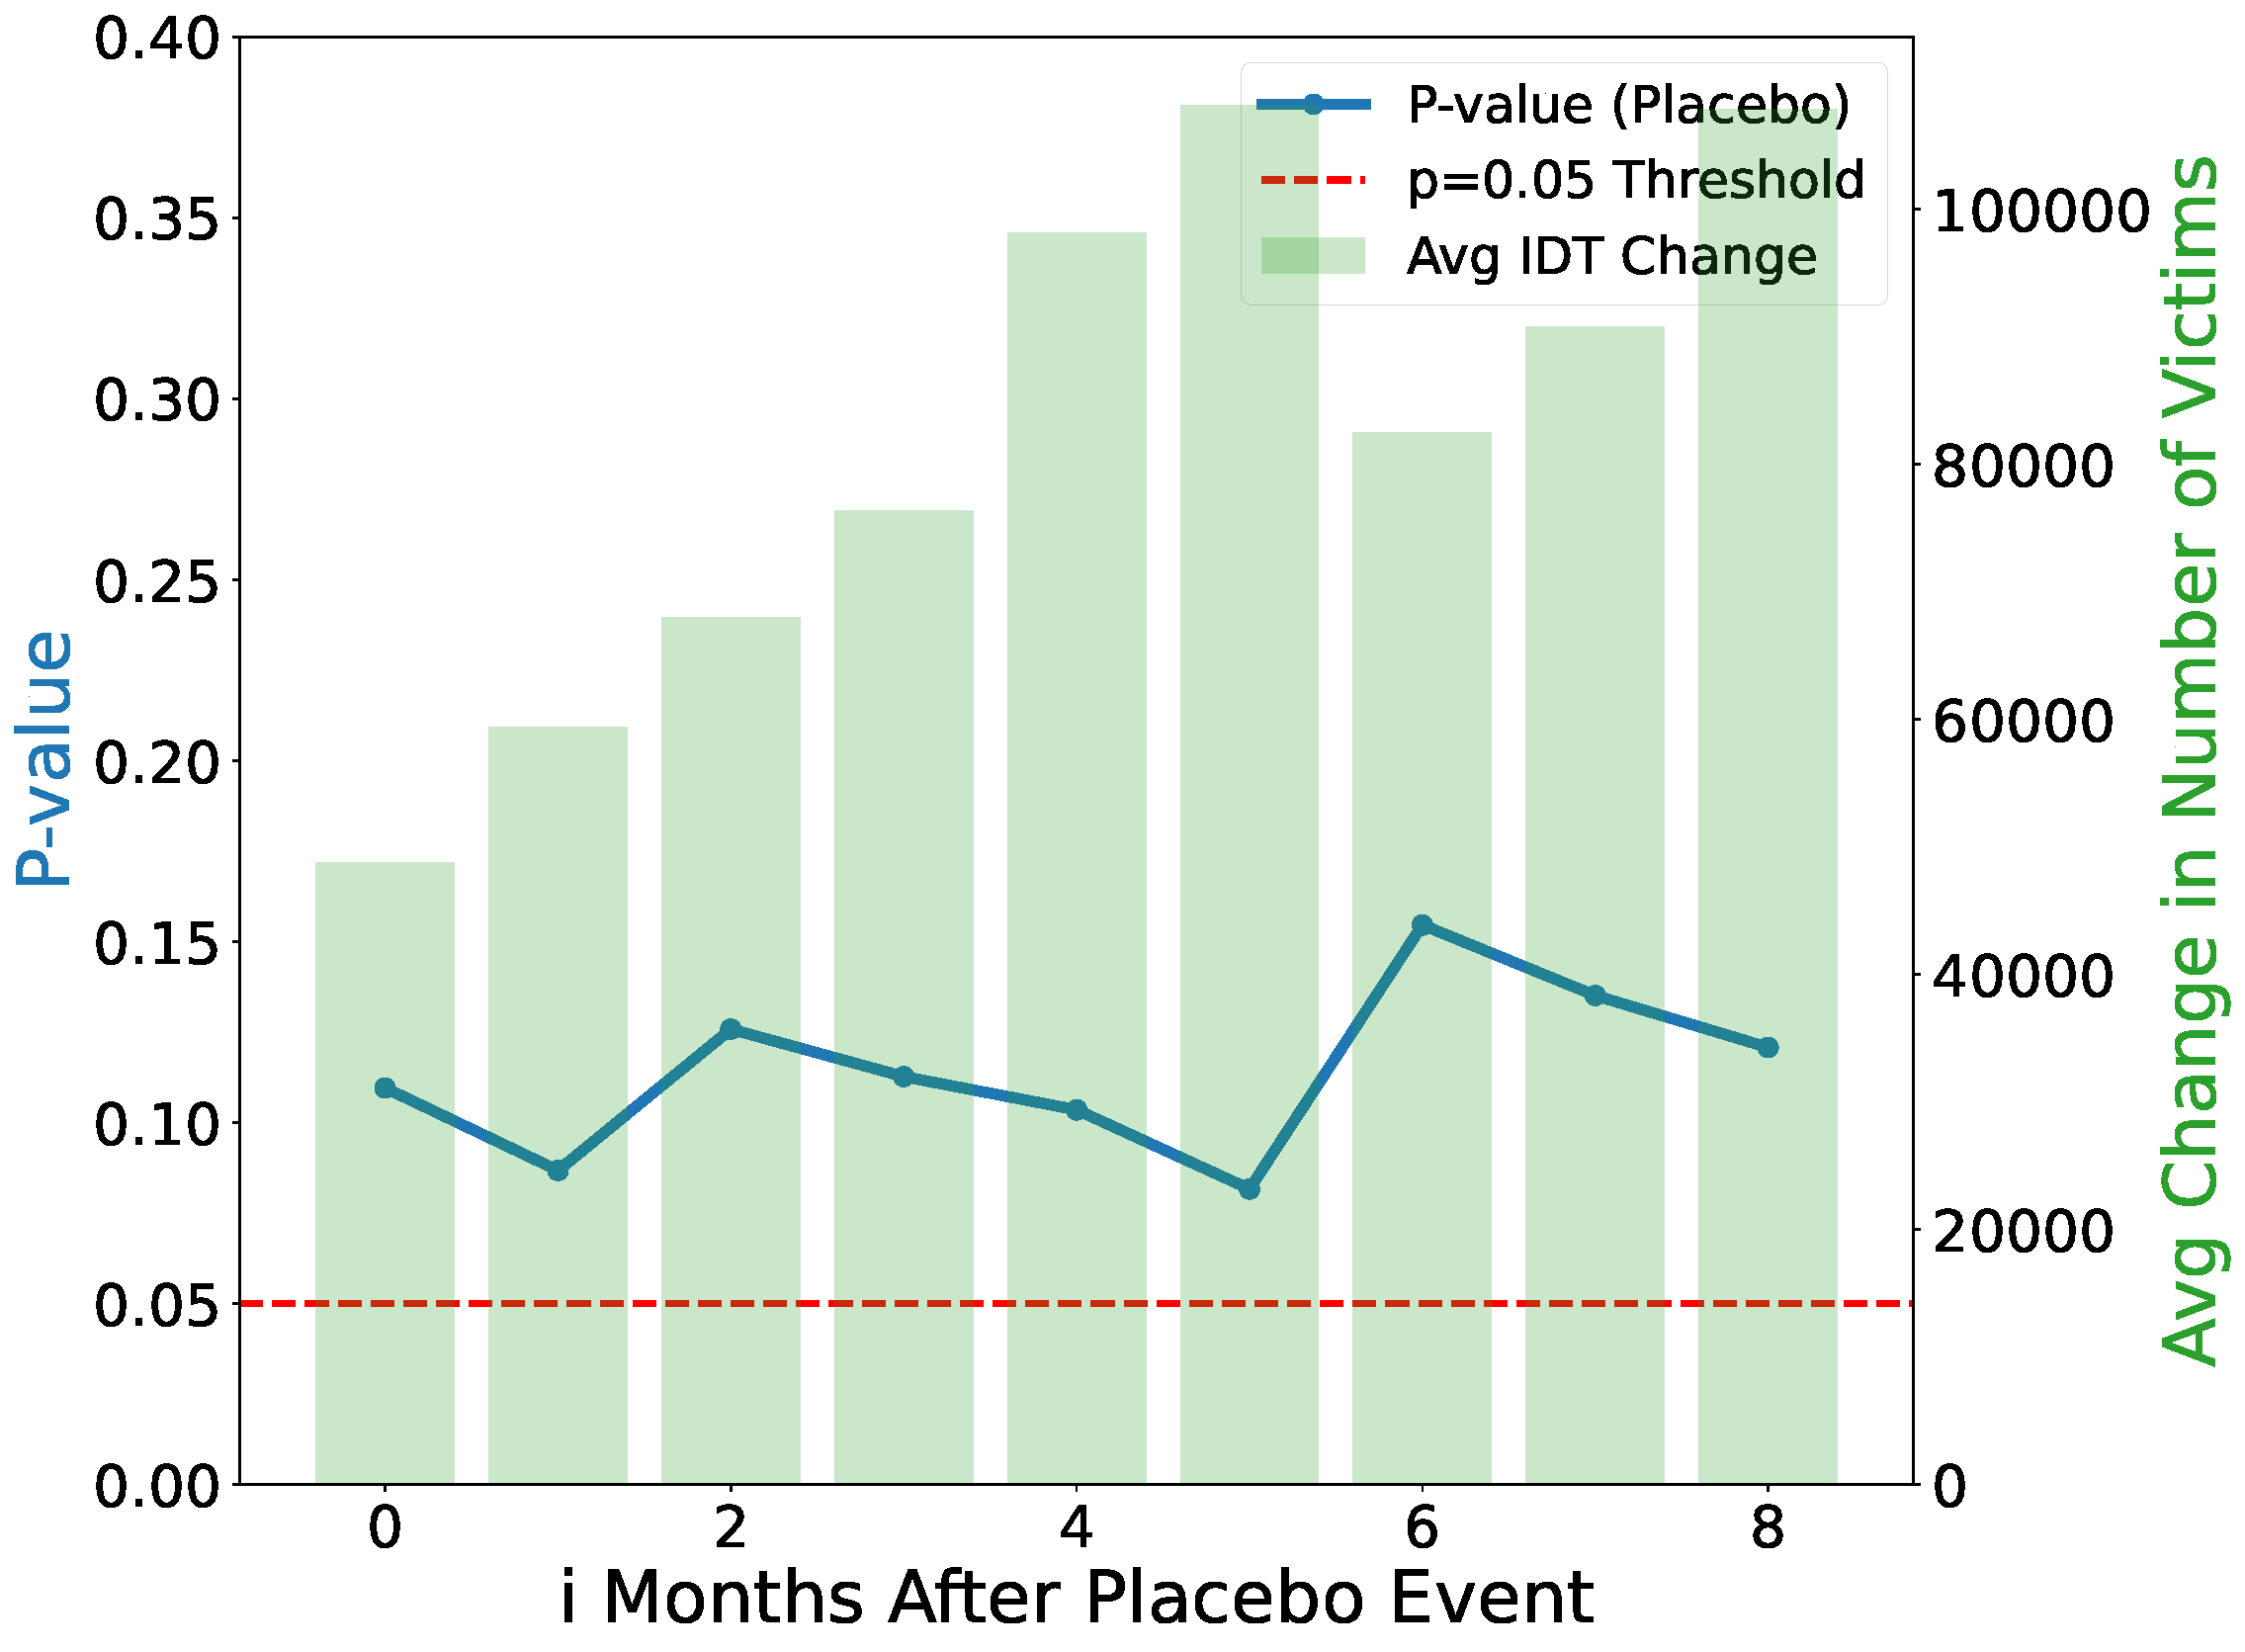
\includegraphics[width=\textwidth]{figures/part6/placebo_longitudinal_sweep_raw_data.pdf}
        \caption{\rev{Placebo (No mega-breach event).}}
        \label{fig:wilcoxon_placebo}
    \end{subfigure}
    
    \caption{Wilcoxon signed-rank test results: Comparison between augmented PRC data and placebo results.}
    \label{fig:wilcoxon_comparison}
\end{figure}

\rev{To validate that the observed spikes are uniquely tied to mega-breaches rather than general trends, we also conducted a placebo test. In this control experiment, we identified all months in our dataset that did not meet the 10 million record mega-breach threshold. We then applied the identical longitudinal sweep methodology to these placebo months, treating them as pseudo-events. Following the same 3-month consolidation rule used for the primary experiment, this identified a set of control points where no major exposure occured. We hypothesized that for these placebo events, the null hypothesis should fail to be rejected across all discovery lags (e.g., we would observe $p > 0.05$).}

The results of the longitudinal sweep \rev{for both the augmented PRC data and the placebo control} are shown in Figure \ref{fig:wilcoxon_comparison}. In \rev{these plots,} the blue line tracks the $p$-value across varying discovery lags, while the green bars indicate the average change in the estimated number of monthly victims (calculated from the ITS  data), compared to the pre-breach baseline. When examining the results in Figure \ref{fig:wilcoxon_raw}, we observe a clear window of statistical significance: the null hypothesis is rejected ($p<0.05$) for discovery lags of 1 and 2 months. The analysis reveals that the lowest $p$-value occurs for a lag of 2 months. During these periods of statistical significance, the estimated number of IDT victims rises by approximately 175,000 to 190,000 individuals per month compared to the pre-breach baseline. Notably, the $p$-value rises above the 0.05 threshold by the third month, suggesting that the shock of a mega-breach on reported victimization levels dissipates relatively quickly. These findings demonstrate a significant, though time-limited, correlation between massive data exposures and surges in IDT reports. \rev{Conversely, the results of the placebo test shown in Figure \ref{fig:wilcoxon_placebo} confirm that when no mega-breach occurs, there is no statistically significant increase in identity theft. Across the entire range of discovery lags ($i \in \{0, \dots, 8 \}$), the $p$-value remains consistently above the 0.05 threshold, often exceeding 0.10.}

The result of this Wilcoxon testing will directly inform how we construct a lower-bound on the estimated social cost of a mega-breach in Section \ref{sec:breach_social_cost}, by focusing exclusively on the immediate aftermath of the breach, indicated by the spike in reported IDT as seen above, even though many of the exposed records may lead to IDTs months and years later, which blends into the background and becomes part of the pre-breach ``median'' of the next event.

% The results from the dynamic saturation model in Figure \ref{fig:wilcoxon_saturated} reinforce these findings. Even after attempting to de-duplicate the record count to represent unique individuals, the statistical significance remains there. In this model, the $p$-value remains below the significance threshold for lags $i=0$ through $i=2$, again identifying the months surrounding the breach as the period of highest risk. The magnitude of the effect is slightly more pronounced in the saturation model, with the average increase in victims peaking at over 200,000 in the second month. Comparing the two figures demonstrates that the correlation between mega-breaches and IDT spikes is significant.

%\com{Maybe some additional clarification would be helpful here: the test itself is done on the IDT data, correct? the PRC data is only used to determine how to slide those windows over the IDT data, no? I know I initially suggested doing this two ways, but now I'm confused why they are not the same...} \resp{Prof. Liu, Yes that is correct. I added some clarification and rewrote this section as per our conversation.}

%\com{We can also vary the definition of a mega event and see what changes..} \resp{Yes, I tried values between 1M-15M, but 10M gave me the best results.}

% For the output of our dynamic saturation model, which attempts to de-duplicate the number of exposed records, we lowered this threshold to 5 million. 
%The total number of events after this consolidation is as follows: 19 for the raw augmented data, and 20 for the data after the saturation model was applied. 

\subsection{A Breach-to-Victim Conversion Model}
\label{sec:conversion_rate}

In reality, the impact of a data breach can be long-lasting: exposed records will remain somewhere on the dark web indefinitely waiting for the next exploiter; many unwitting consumers whose records were exposed in breaches never bother to take appropriate actions such as updating their passwords or freezing their credit. In this section we develop a model that attempts to capture this long-term impact, and this model will then directly inform the construction of an upper-bound estimate of the social cost of a mega-breach in Section \ref{sec:breach_social_cost}.

Figure \ref{fig:section7_fig5} shows the monthly counts for both records exposed (the augmented PRC data, in orange) and reported IDT victims (the processed ITS data, in teal). 
%In this overlay, the record count (represented in orange) is derived from our augmented PRC data, while the successful IDT count (represented in teal) is sourced from the processed ITS data. 
Unlike cumulative metrics often found in industry reports, these figures represent month-to-month totals, allowing for a direct comparison of how record exposure spikes correlate with surges in reported IDTs over time (detailed in Section \ref{sec:wilcoxon_methods}). We specifically highlight three mega-breaches: Heartland Payment Systems (January 2009 \cite{USCourts_Heartland}), Target (December 2013 \cite{Target_Breach}), and Equifax (September 2017 \cite{House_Equifax}). These three incidents appear as prominent spikes on the record exposure curve in Figure \ref{fig:section7_fig5}. As can be seen, while the volume of exposed records exhibits volatility over the 13-year study period, it is generally increasing over time. 
The number of successful IDT reports follows a more stable trajectory. 

\begin{figure}[htbp]
    \centering
    \begin{minipage}[t]{0.48\textwidth}
        \centering
        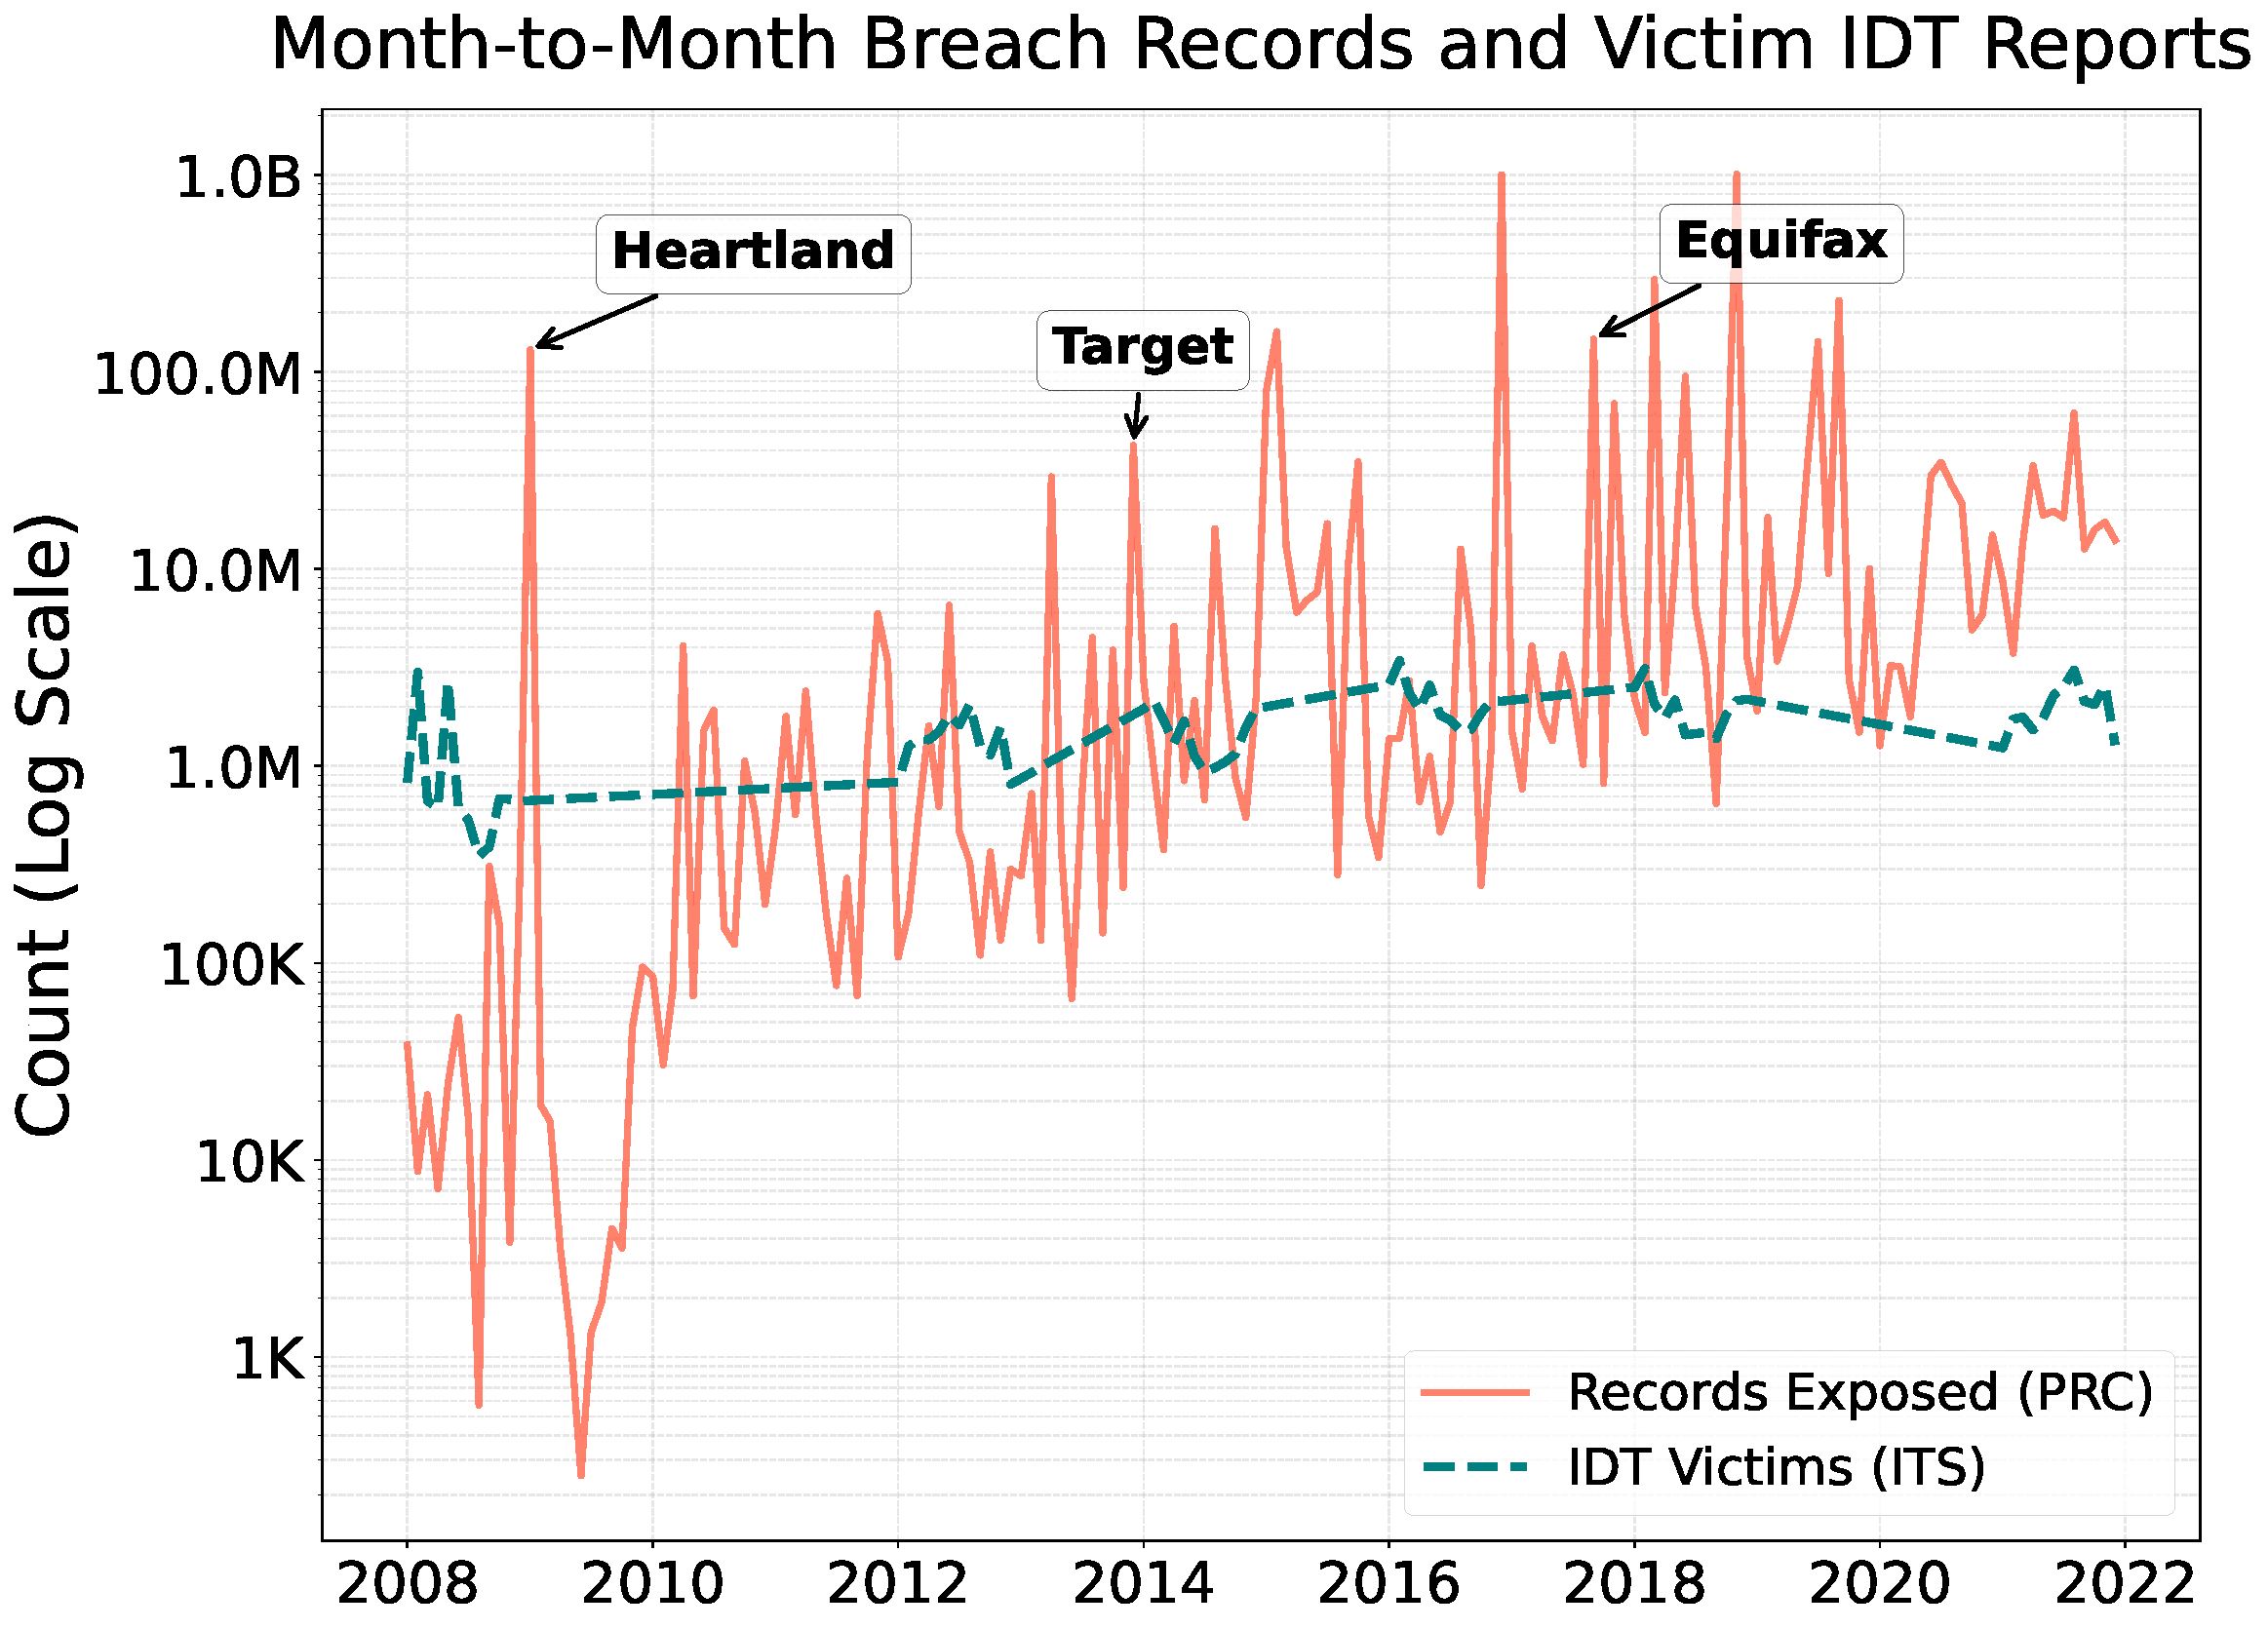
\includegraphics[width=\textwidth]{figures/part5/overlay_raw.pdf}
        \caption{Number of records exposed (PRC) and number of reported IDT victims (ITS) over the study period.}
        \label{fig:section7_fig5}
    \end{minipage}
    \hfill 
    \begin{minipage}[t]{0.47\textwidth}
        \centering
        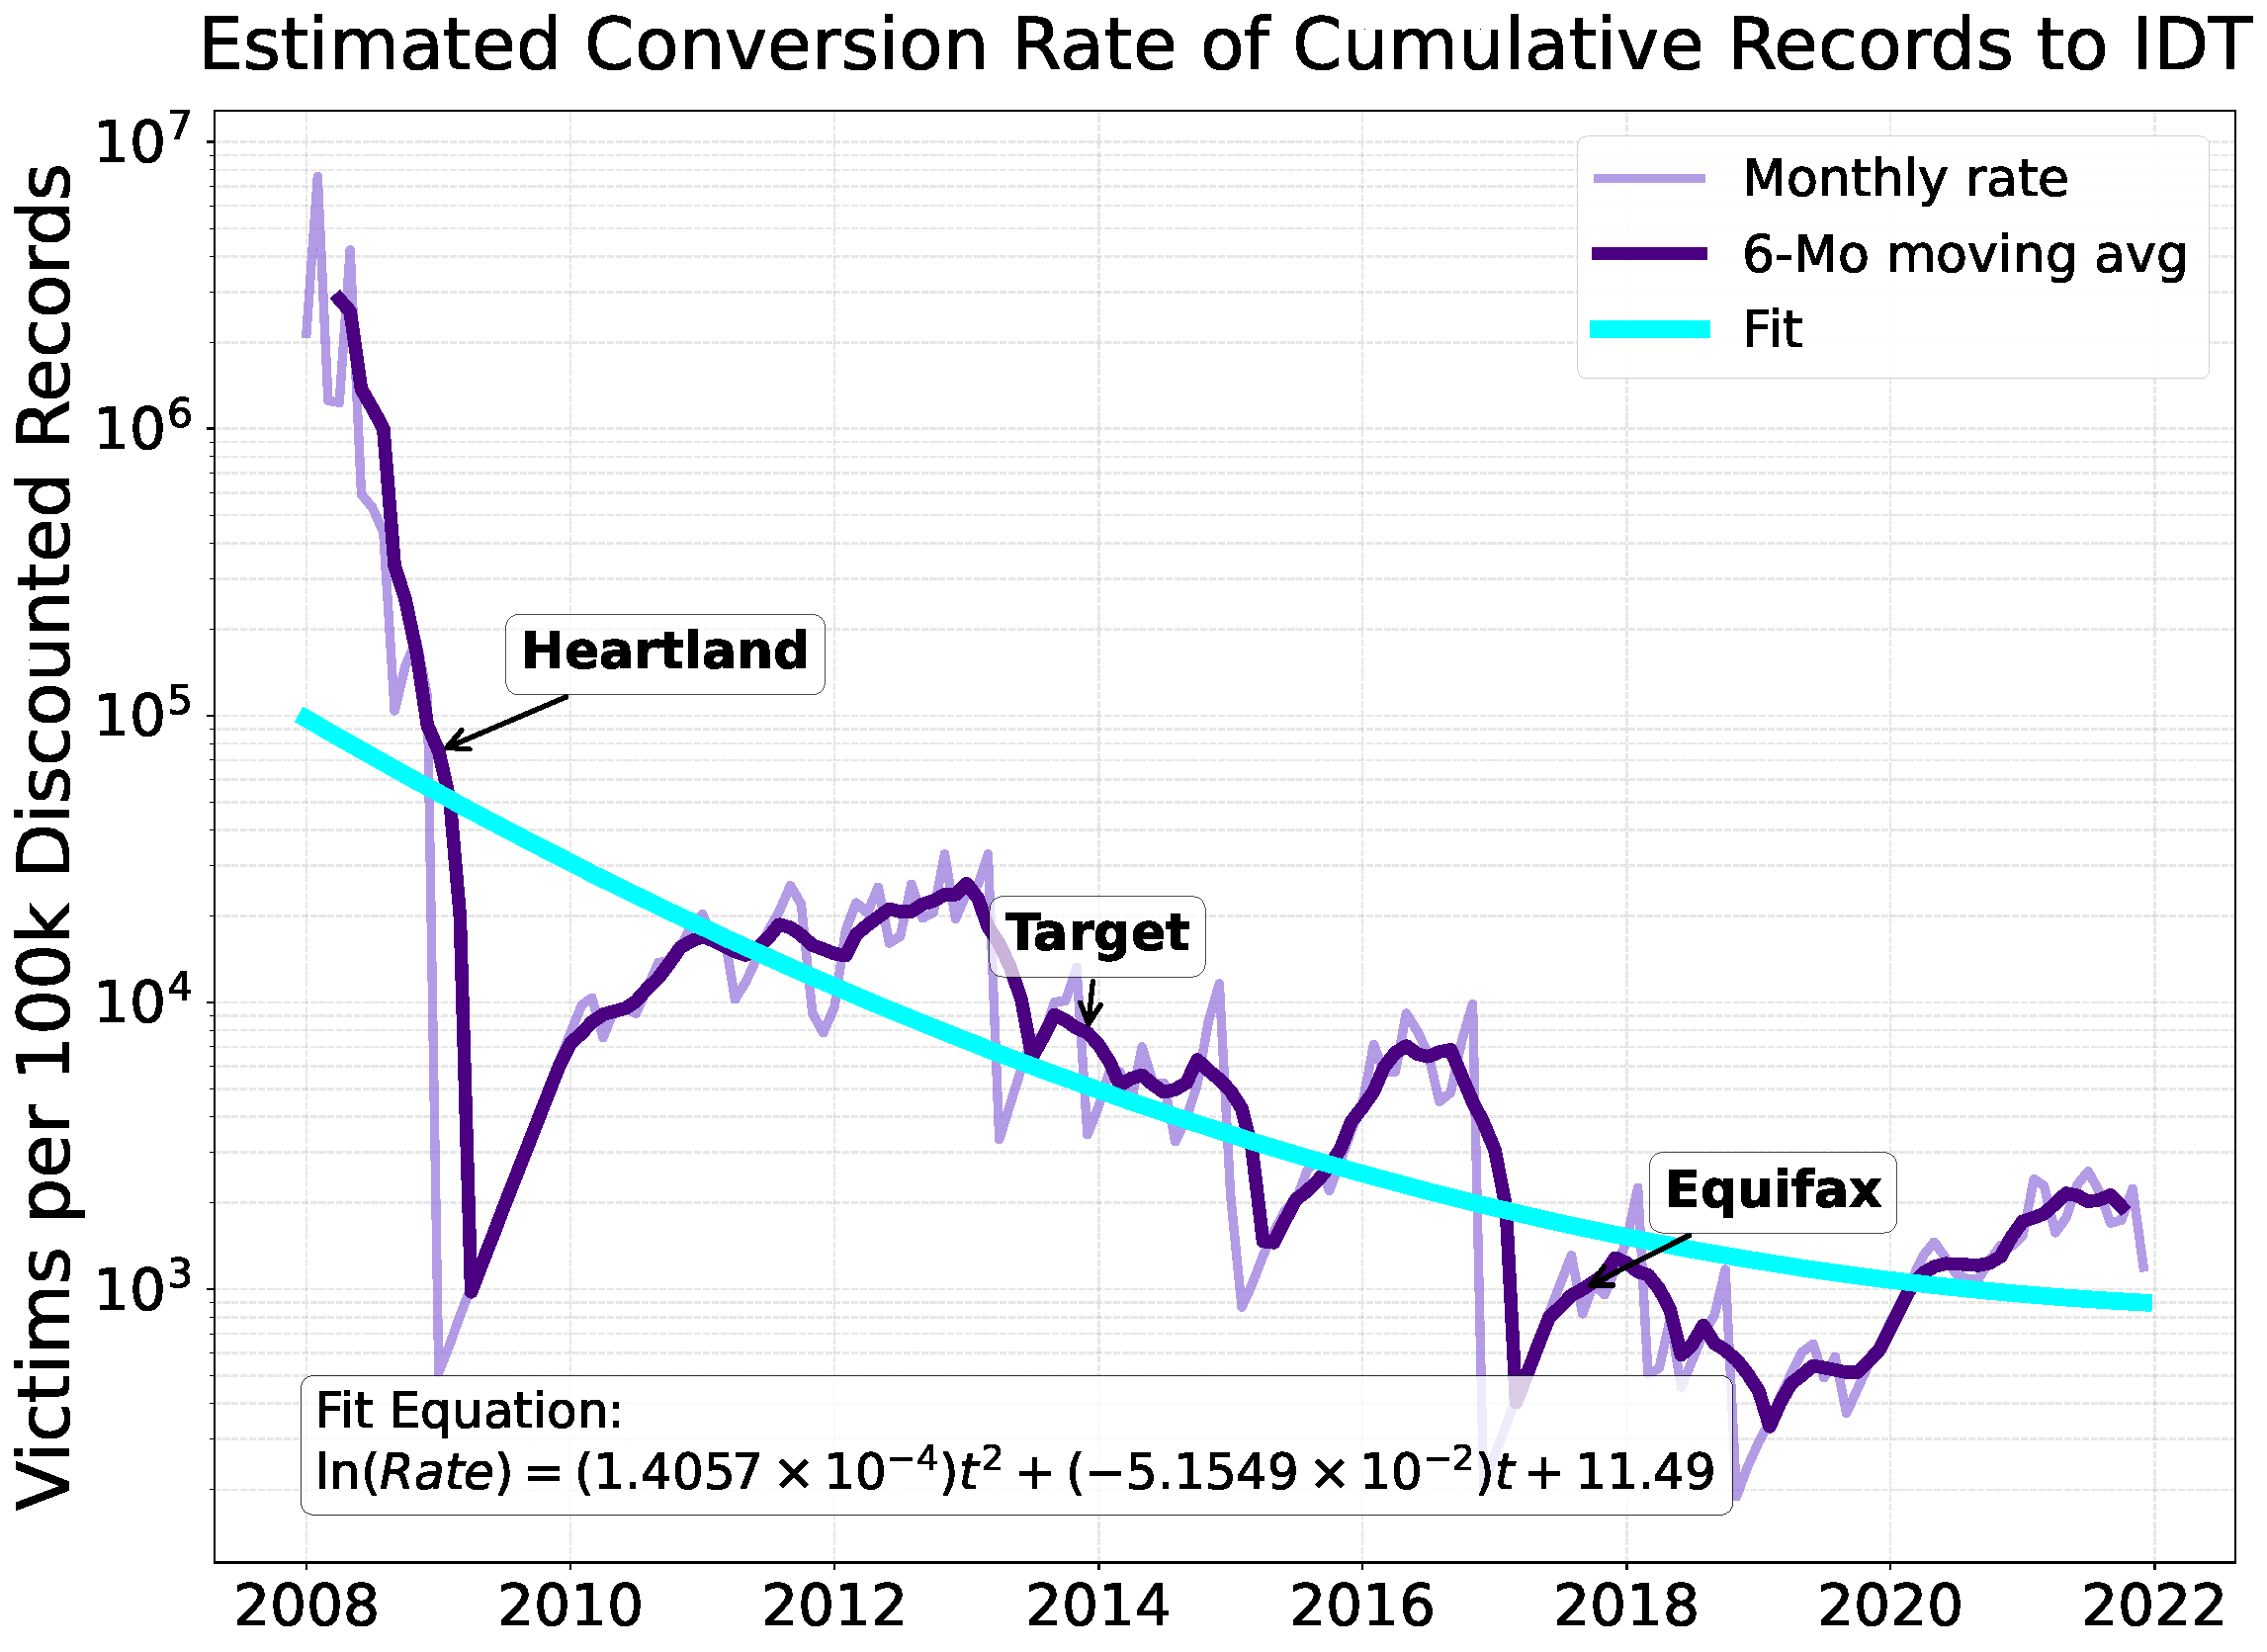
\includegraphics[width=\textwidth]{figures/part5/conversion_rate_beta.pdf}
        \caption{Analysis of conversion rates from data being breached to becoming an IDT victim. }
        \label{fig:conversion_rate}
    \end{minipage}
    
\end{figure}



We define an estimated conversion rate of cumulative breached records (up to month $t$) to IDT (in month $t$), denoted by $\mathcal{C}_t$. Here, $t$ represents the number of months since the start of the study period ($t=0$ for January 2008). This method acknowledges that IDT in any given month is rarely the result of a single isolated breach; rather, it is drawn from a longitudinal supply of previously compromised records that remain ``fresh'' or exploitable on the criminal market. We assume that compromised/stolen data has an infinite ``shelf-life'' but with diminishing utility over time as victims change passwords, credit cards expire, or financial institutions improve fraud detection. To model this, we define the total available pool of exposed data at time $t$ as a discounted cumulative sum, $D_t$, calculated recursively as follows, where $M_k$ represents the monthly record exposure for month $k$ (from the augmented PRC dataset) and $\alpha$ is a discount factor representing the decreasing utility of stolen data over time: 
\begin{equation}D_t = \sum_{k=0}^{t} \alpha^{t-k} M_k~. 
\end{equation}
In our experiments we will set $\alpha = 0.8$, which implies that roughly 20\% of the utility of a leaked record is lost each month. It should be noted that this particular choice of the discount factor value, while arbitrary, is not critical: this modeling step is followed by a regression (discussed shortly below), so any change in this choice will largely be compensated by the fit equation. This is because the log-quadratic regression essentially treats $\alpha$ as a scaling parameter; while different discount factors may shift the absolute magnitude of the available data pool, they do not fundamentally alter the longitudinal trend of the conversion rate.

The conversion rate is then expressed as the number of reported victims (from the ITS data) at time $t$ for every 100,000 discounted cumulative records available on the market by month $t$. 

\begin{equation}\mathcal{C}_t = \frac{\text{(Number of IDT Victims)}_t}{D_t} \times 100,000~. 
\end{equation}

The results of applying this model are shown in Figure \ref{fig:conversion_rate}, where we calculated this conversion rate at monthly intervals (light purple) and applied a six-month moving average (dark purple) to identify long-term trends. Again, we explicitly highlight the Heartland, Target, and Equifax breaches as consistent reference points to allow for a direct comparison between raw record exposure in Figure \ref{fig:section7_fig5} and conversion rate in Figure \ref{fig:conversion_rate}. The localized peaks in the conversion rate primarily coincide with the ITS survey waves. This suggests that the volatility is largely driven by the periodic transition from interpolated victim estimates back to raw weighted survey data.
%\com{out of curiosity, what are some of the peaks on the dark purple curve.. are those also mega breaches?} 
%\resp{I actually think this has more to do with the ITS data being more available at these times (and not being interpolated)... but let me look into this more} \resp{Confirmed, i added a sentence above that says that, but we can take it out if needed.}
The conversion rate in Figure \ref{fig:conversion_rate} exhibits a generally decreasing trend; as the cumulative pool of stolen data $D_t$ grows by orders of magnitude, the marginal ``yield'' or criminal value of a single record decreases. This is also reflected in Figure \ref{fig:section7_fig5}, where the volume of records exposed in later years is significantly higher than in initial years; however, because the number of successful IDTs did not grow at a matching rate, the resulting conversion rate dropped.


% Note that in Figure \ref{fig:conversion_rate}, the conversion rate early in the study period sits above the 1:1 ratio, which is the $y = 10^5$ line (representing 100,000 victims per 100,000 records breached). The reason for this is evident in Figure \ref{fig:section7_fig5}, where the orange curve representing breached records is lower than the teal curve representing IDTs during those years. This \rev{likely} indicates that while the PRC database had more limited coverage of breach events in the early years, the ITS survey was still capturing a steady amount of national victimization. As the study period progresses, in later years, the volume of breached records (the orange curve in Figure \ref{fig:section7_fig5}) increases, and we see the conversion rate in \ref{fig:conversion_rate} decrease to the 1:1 ratio and then decrease below it.


% Furthermore, Figure \ref{fig:conversion_rate} displays a sharp spike in conversion rate after the Heartland Payment Systems breach in 2009. This could be due to the high utility and low saturation of the stolen data market at that time; with less stolen data available to criminals in 2009, the ''yield'' of a single compromised record was higher. We do not observe the same magnitude of this trend for the 2013 Target or 2017 Equifax breaches. This could be because by these later dates, the national supply of stolen personal information had begun to reach saturation. As illustrated in Figure \ref{fig:section7_fig5}, the volume of records exposed in these later years increased by orders of magnitude; however, because the number of successful IDTs did not grow at a matching rate, the resulting conversion rate dropped. 

To model this trend for our purpose, %predictive use, 
we performed a time-based log-quadratic regression on the six-month moving average. This model estimates the expected conversion rate as a function of time $t$, where $t$ is again defined as the number of months since January 2008. The resulting fit equation is:
\begin{equation}
\label{eqn:fit}
    \ln(\mathcal{C}_t) = (1.41 \times10^{-4})t^2 + (-5.15 \times 10^{-2})t + 11.49~. 
\end{equation}

To retrieve the (instantaneous) conversion rate $\mathcal{C}_t$ for a breach, we first calculate the $t$ value (months after January 2008) for the breach given its date. Plugging this $t$ value into Equation \ref{eqn:fit} and taking the exponential (to undo the natural logarithm) yields the conversion rate for that specific breach. For example, the conversion rates at the times of the Heartland  ($t=12$), Target ($t=71$), and Equifax ($t=116$) breaches were 75,205, 7,841, and 1,001 IDT victims per 100,000 discounted exposed records, respectively.

In this model, the negative linear coefficient ($-5.15 \times 10^{-2}$) represents the overall downward trend on conversion rate over time, likely due to improved fraud detection systems. The quadratic coefficient ($1.41 \times10^{-4}$) accounts for the slight flattening of the curve in recent years, reflecting a stabilizing risk. Equation \ref{eqn:fit} allows us to estimate the expected victim yield for specific breach events based on their historical timing. We will use this model in Section \ref{sec:breach_social_cost} to provide upper-bound estimates on the social costs of specific breach events. 
%for the three mega-breach events highlighted in Figures \ref{fig:section7_fig5} and \ref{fig:conversion_rate}.
%\com{Did we ever try the conversion rate calculated as victim in month $t$ over records exposed in month $(t-2)$?} \resp{Prof. Liu, yes we did. But it did not change much other than decreasing the quadratic coefficient by a little. }


% Figure \ref{fig:section7_fig5} illustrates the monthly trends for both the estimated number of \rev{unique} records exposed and the total count of reported IDT victims. While the volume of exposed records exhibits extreme volatility, often driven by extremely large-scale breaches involving hundreds of millions of records, the number of successful IDTs follows a slightly increasing trajectory. 

% \com{Consider flipping the roder of these two figures if Fig 5 is mentioned before Fig 4..}



%% SATURATION MODEL BELOW
% To quantify the risk posed by these breaches, we calculated the breach to IDT victim conversion rate, defined as the number of successful IDT victims per 100,000 \rev{estimated exposed unique records}. \rev{Following our model above, we applied the dynamic saturation model to adjust for the 16+ population to de-duplicate and count how many unique individuals are placed at risk relative to the aggregate record volume.} \com{Are there other mathematical details here that we should spell out?} Figure \ref{fig:conversion_rate} displays this rate over the 13-year study period, along with a six-month rolling average to identify long-term trends. Our analysis reveals a \rev{mostly stable trend} in the conversion rate over time, \rev{with a slight overall downward trend over the long-term, especially in more recent years}. In early years of the study, the rate frequently peaked near $10^5$, suggesting a high efficiency in converting stolen data into successful fraud. \rev{Following an initial decline as the market moved towards saturation, Figure \ref{fig:conversion_rate} displays the rate maintaining a position between $10^4$ and $10^6$ victims per 100,000 unique records exposed. } This suggests that while the volume of record exposure is reaching high levels, \rev{the relative efficiency with which criminals use unique credentials remains high.} In addition, as shown in our longitudinal analysis in Appendix \ref{app:longitudinal}, \rev{the interplay between} better monitoring \rev{and evolving criminal tactics creates a persistent level of risk.} These findings directly tie into our social cost estimate. \rev{Furthermore, the slight decreasing trend could be due to saturation of the data market.} While the conversion rate varies, the magnitude of record exposure ensures that the total social harm remains high. Even a \rev{stable} conversion rate applied to millions of exposed records results in large numbers of victims, who each have to face the social cost of their IDT.
% \com{Did we end up using the conversation rate in the next subsection, or did we simply use the incident-specific data?}

% \com{there is an alternative way of doing this which does not involve messing with the raw data.. we can simply take the cumulative raw counts and the IDT counts (smoothed), plot the down conversion rates between the two and do a quadratic curve fit.. }




\subsection{The Social Cost of Mega-breaches}
\label{sec:breach_social_cost}
To apply our social cost model to real-world mega-breach events, we performed an analysis of the three landmark security events highlighted earlier: the 2009 Heartland Payment Systems breach, the 2013 Target breach, and the 2017 Equifax breach. We chose these three incidents because they were large breaches that compromised significant portions of the U.S. population (around 130 million for Heartland \cite{USCourts_Heartland}, around 40 million for Target \cite{Target_Breach}, and around 147 million for Equifax \cite{House_Equifax}), and because they have well documented corporate settlement figures that allow direct comparison with our social cost estimates. For each of these case studies, we establish both a lower bound and an upper bound estimate. 

\begin{enumerate}[label=(\alph*)]
\item \textbf{Lower Bound (Empirically Measured Short-Term Impact):} This estimate utilizes the Wilcoxon-signed rank analysis presented earlier to measure the statistically significant increase in IDT victims discovered in the 6-month window (with a discovery lag of $i=2$) immediately following the breach. This essentially means if a breach occurred at time $t$, we measure the average increase in IDT victims in months $t+2$ to $t+8$.
By multiplying the increase in number of measured identity victims post-breach with the social cost per victim at the time of the breach, we calculate an estimate of the breach's social cost. This is a lower-bound estimate because it is based on the short-term impact of the breach empirically measured by the increase in the number of victims immediately following the breach. 

\item \textbf{Upper Bound (Projected Long-Term Impact)}: This estimate utilizes our log-quadratic fit (Equation \ref{eqn:fit}) and the discount factor $\alpha = 0.8$ to project the total victim yield for a specific breach as well as the life-time cost incurred by the breach. To maintain consistency with our empirical findings, the projection begins after a discovery lag of two months. For a breach of size $B$ that occurred at time $t$, the remaining ``fresh'' records from the breach is estimated to be $B \cdot \alpha^{k-t}$ from month $k=t+2$ through the end of the study period; applying to this the monthly conversion rate $\mathcal{C}_k$ we obtain the estimated number of victims in month $k$ attributed to the breach; summing up these estimates then gives us the projected total number of victims over the long term. By weighting the monthly victim yield by an interpolated monthly social cost of IDT $S_k$, we obtain the estimated social cost in month $k$ attributed to the breach. Summing these values across the study period then provides the total projected social cost of the incident over the long-term. 
%
This serves as an upper bound because it accounts for the victimization that extends beyond the immediate post-breach shock, assuming the conversion of stolen records encompasses the full scale of the exposure over time.

% To have a consistent comparison with our lower bound estimate, we average the conversion rate over the six months following a breach, with a discovery lag of $i=2$. This essentially means that if a breach occurred at time $T$, we measure the average  conversion rate during months $T+2$ to $T+8$. By applying this rate to the number of records exposed in a breach, we estimate the total potential number of victims resulting from that breach, and then multiply this number of estimated victims by the social cost per victim at the time of the breach. This serves as an upper bound estimate because it accounts for the stolen data market's volume of exposed records. Unlike the lower bound estimate, which is limited to only capturing the immediate, measured surge in reported IDT victims, this projection assumes that the conversion of stolen records into IDT encompasses the full scale of the exposure.


%\com{I like your attempt to justify why this is an upperbound :-), though I am not sure it's fully convincing...} \resp{Haha, I am trying hard to justify it, but the only real reason I think it is an upper bound is that its simply very high...}
\end{enumerate}

\subsubsection{The Lower Bound Estimate}
For our lower bound estimate, we calculated the change in the number of IDT victims statistically attributable to each breach. This was derived from the Wilcoxon signed-rank test as described in Section \ref{sec:wilcoxon_methods},  using a discovery lag of 2 months. We compared the median monthly victimization count in the six months prior to the breach against the median monthly victimization count in the six months immediately following the breach with a two-month delay in between. The difference between these two periods represents the estimated increase in victim count that coincides with the breach window. 
%
For each breach, we identified the statistically significant victim count increase following the breach. We then translated these victim counts into the  cost estimate by multiplying the social cost data from Table \ref{tab:social_costs_by_year}:  %Overall, the social cost calculation was done as follows: 
$$\text{Total Social Cost} = \text{Social Cost per Victim} \times \text{Number of Victims}$$

Using the social cost per victim from the years closest to the incidents, we noted \$1,110.31 for the 2008 period for the Heartland breach, \$853.41 for the 2014 period for the Target breach, and \$244.40 for the 2018 period for the Equifax breach. 
More specifically, 
\begin{enumerate}
\item For the Heartland breach, our analysis identified a statistically significant median increase of 88,956 victims per month in the post-breach window. Multiplying this by the six-month observation period and the 2008 social cost per victim of \$1,110.31 yields a total social cost of approximately \$592.7 million. Compared to its cumulative \$107 million settlement \cite{heartland_amex_2009, heartland_mastercard_2010, heartland_visa_2010, heartland_consumer_2012}, the social cost was over five times higher than the institutional payout.

\item For the Target breach, our analysis identified a statistically significant median increase of 59,714 victims per month, resulting in an estimated 358,284 total victims in the post-breach window compared to the pre-breach baseline. Applying the \$853.41 social cost per victim from the 2014 period results in a total estimated social cost of approximately \$305.8 million.  In contrast, Target's highly publicized multi-state settlement for the breach was only \$18.5 million \cite{TexasAG_TargetSettlement}. This indicates that the realized social harm was about 18 times higher than the institutional payout. 

 % Applying this formula to the Target breach results in a total estimated social harm of approximately \$241 million. When divided by the 40 million records exposed, this yields a realized social cost of \$6.03 per record.
%\com{I wonder whether it makes more sense to do this this way (breach-specific increases) or simply use an average increase across all mega-breaches..}

\item For the Equifax breach, our analysis found a median increase of 179,889 victims per month, leading to an estimated 1,079,334 victims following the breach. Using the \$244.40 social cost per victim from the 2018 period, the estimated total social cost is \$263.8 million. Despite the severity of this exposure, Equifax's global settlement was capped at \$700 million \cite{FTC_EquifaxSettlement}. In this specific instance, the compensation settlement actually exceeded the estimated immediate social costs. This reversal, where the settlement exceeds the estimated social costs, may reflect the saturation effect observed in our earlier analysis. By 2017, many victims were likely already compromised, reducing the marginal impact of a new breach. 
\end{enumerate}

% For the Equifax breach, the social cost per victim in 2016 resulted in an estimated total social cost of \$44.1 million, or roughly \$0.30 per record. 



We acknowledge that this methodology relies on the attribution of a change in the number of IDT victims to specific breach events. By isolating the specific window surrounding a breach, we have attempted to provide a  causal estimate. It is also important to note that our current model treats all compromised records as equal units of risk, yet we know that breaches involving sensitive personal information such as SSNs inherently carry a higher potential for long-term damage than those involving changeable credentials like credit card numbers. While our analysis in the Appendix \ref{app:social_cost_breach} briefly touches on the higher costs associated with SSN exposure, the case study calculations above do not apply a specific weight to the breached records that reflects how sensitive the records are. Future refinements of this model should aim to quantify this distinction, as the lower social cost for Equifax may mask a higher cost due to SSN exposure.


\subsubsection{The Upper Bound Estimate}
The upper bound victim yield for a breach occurring at time $t$ is calculated by summing the anticipated victim yield over the remaining months of the study period. As detailed in \ref{sec:conversion_rate}, this approach assumes that every compromised record has a utility that decays as security measures are implemented or the data becomes stale. We use the same discount factor $\alpha = 0.8$ assumed in \ref{sec:conversion_rate} to represent the monthly retention of a record's exploitative value. To maintain consistency with our empirical findings regarding discovery lags in \ref{sec:wilcoxon_methods}, the projection begins accumulating victims at month $t+2$. The total projected victims for a breach of size $B$ occurring at time $t$ is defined as \rev{$\mathcal{V}_B$}: 

\begin{equation}
    \mathcal{V}_B = \sum_{k=t+2}^{T} (B \cdot \alpha^{k-t}) \cdot \frac{\mathcal{C}_k}{100,000}~, 
\end{equation}
where $\mathcal{C}_k$ is the instantaneous or immediate conversion rate at month $k$, defined from our log-quadratic fit (Equation \ref{eqn:fit}), and $T$ is the terminal month of the study period ($T=167$, December 2021). 
We then multiply this number of projected victims by a time-varying social cost $S_k$ as follows:
% This number of projected victims is then multiplied by the social cost per victim (from Table \ref{tab:social_costs_by_year}) at the time of the breach. 
%
\begin{equation}
\label{eq:social_cost_breach_upper}
\text{Total Estimated Social Cost} = \sum_{k=t+2}^{T} \left( B \cdot \alpha^{k-t} \cdot \frac{\mathcal{C}_k}{100,000} \cdot S_k \right)~, 
\end{equation}
where $S_k$ is the social cost per victim in month $k$, derived through linear interpolation of the social cost estimates presented in Table \ref{tab:social_costs_by_year}. Because the ITS only provides specific survey years, we utilized a piecewise linear function to estimate the social cost for intervening months. This approach acknowledges that the factors influencing social cost, such as the efficacy of bank fraud detection and the value of lost time, shift gradually over time rather than in abrupt annual steps. By embedding this time-varying social cost into our summation, we ensure that victims occurring later are valued at the contemporary victim social cost relevant to their time of discovery, rather than a static cost fixed at the date of initial record exposure. 

% \resp{Below paragraph needs updating to reflect changes above}

Applying this model to our three landmark mega-breaches, we obtain the following: 
%reveals a significant gap between corporate settlements and total projected social harm. 
\begin{enumerate}
\item For the 2009 Heartland Payment Systems breach, the model projects approximately 171.8 million victims resulting from the mega-breach event. %Multiplying by the time-decaying social cost of IDT 
\rev{Using Equation \ref{eq:social_cost_breach_upper}, we obtain an upper bound social cost estimate of the Heartland breach at} \$179.1 billion, which is approximately 1,673 times higher than Heartland's cumulative settlement of \$107 million \cite{heartland_amex_2009, heartland_mastercard_2010, heartland_visa_2010, heartland_consumer_2012}.  This reflects the vulnerability of a breached record in early years, where a single record has a high probability of successful conversion into financial crime. 

\item For the 2013 Target breach, we estimate a projected yield of 5.49 million victims and an upper bound social cost of \$4.06 billion. This figure is over 219 times higher than Target's \$18.5 million settlement \cite{TexasAG_TargetSettlement} highlighting how the majority of social costs are externalized onto the public. 

% Combined with the high per-victim cost of \$1,110.31 from the 2008 period, the resulting upper bound social cost is \$190.7 billion, roughly 1,362 times higher than 

% \item 
% Using the 2012 social cost per victim of \$921.38, the total projected social harm is \$5.06 billion. 

\item 
Finally, for the 2017 Equifax breach, the model projects 6.95 million victims resulting from the breach. Despite the high volume of records exposed in this breach (147 million), the increased market saturation and improved fraud detection in 2017 results in a lower per-record victim yield than in previous years. Our upper bound estimated social cost for the Equifax breach is \$1.72 billion. This projection still more than doubles Equifax's \$700 million settlement cap \cite{FTC_EquifaxSettlement}, suggesting that even in a saturated market, the long-term impact of data exposure can create a multi-billion dollar social burden.

% Multiplying these victims by the \$245.27 per-victim cost from the 2016 period yields an upper bound social cost of \$1.70 billion. 


\end{enumerate}

\subsubsection{Summary}
A summary of our upper and lower bound estimates is displayed in Table \ref{tab:case_study_summary}, where we see a profound disparity between corporate liability and realized social harm, \rev{even when this harm is rather narrowly defined}. In two out of the three case studies (Heartland and Target), even our lower bound social cost estimate (which only captures the short-term impact) exceeded the breach's settlement. The upper bound projections reveal a far more severe social cost, as the projected long-term impact from the Heartland, Target, and Equifax breaches exceeded their respective settlements by factors of approximately 1,673, 219, and 2.

These results also provide empirical evidence of the saturation effect within the stolen data market. While the total number of records exposed in the 2017 Equifax breach was greater than that of the 2009 Heartland breach, the projected social harm for Equifax is two orders of magnitude lower. This decline in marginal yield reflects the diminishing utility of new data as the national supply of compromised identifiers reaches saturation. Nevertheless, the \$1.72 billion upper bound social cost for Equifax still more than doubles the \$700 million settlement cap, suggesting that the long-term exposure of data in even a saturated market imposes a persistent financial burden on the consumer that current regulatory penalties fail to fully address.


\begin{table}[h]
\centering
\caption{Comparison of Corporate Settlements and Estimated Social Costs for Mega-Breach Events}
\label{tab:case_study_summary}
\begin{tabular}{lcccccc}
\hline
\textbf{Case Study} & \textbf{Date} & \textbf{$t$} & \textbf{Records ($M$)} & \textbf{Settlement} & \textbf{Lower Bound} & \textbf{Upper Bound} \\ \hline
Heartland & 2009-01 & 12 & 130.0 M& \$107 M & \$592.7 M & \$179.1 B \\
Target & 2013-12 & 71 & 40.0 M& \$18.5 M & \$305.8 M & \$4.06 B \\
Equifax & 2017-09 & 116 & 147.0 M& \$700 M & \$263.8 M & \$1.72 B \\ \hline
\end{tabular}
\end{table}